\PassOptionsToPackage{unicode=true}{hyperref} % options for packages loaded elsewhere
\PassOptionsToPackage{hyphens}{url}
%
\documentclass[]{article}
\usepackage{lmodern}
\usepackage{amssymb,amsmath}
\usepackage{ifxetex,ifluatex}
\usepackage{fixltx2e} % provides \textsubscript
\ifnum 0\ifxetex 1\fi\ifluatex 1\fi=0 % if pdftex
  \usepackage[T1]{fontenc}
  \usepackage[utf8]{inputenc}
  \usepackage{textcomp} % provides euro and other symbols
\else % if luatex or xelatex
  \usepackage{unicode-math}
  \defaultfontfeatures{Ligatures=TeX,Scale=MatchLowercase}
\fi
% use upquote if available, for straight quotes in verbatim environments
\IfFileExists{upquote.sty}{\usepackage{upquote}}{}
% use microtype if available
\IfFileExists{microtype.sty}{%
\usepackage[]{microtype}
\UseMicrotypeSet[protrusion]{basicmath} % disable protrusion for tt fonts
}{}
\IfFileExists{parskip.sty}{%
\usepackage{parskip}
}{% else
\setlength{\parindent}{0pt}
\setlength{\parskip}{6pt plus 2pt minus 1pt}
}
\usepackage{hyperref}
\hypersetup{
            pdfborder={0 0 0},
            breaklinks=true}
\urlstyle{same}  % don't use monospace font for urls
\usepackage[margin=1.0in]{geometry}
\usepackage{graphicx,grffile}
\makeatletter
\def\maxwidth{\ifdim\Gin@nat@width>\linewidth\linewidth\else\Gin@nat@width\fi}
\def\maxheight{\ifdim\Gin@nat@height>\textheight\textheight\else\Gin@nat@height\fi}
\makeatother
% Scale images if necessary, so that they will not overflow the page
% margins by default, and it is still possible to overwrite the defaults
% using explicit options in \includegraphics[width, height, ...]{}
\setkeys{Gin}{width=\maxwidth,height=\maxheight,keepaspectratio}
\setlength{\emergencystretch}{3em}  % prevent overfull lines
\providecommand{\tightlist}{%
  \setlength{\itemsep}{0pt}\setlength{\parskip}{0pt}}
\setcounter{secnumdepth}{0}
% Redefines (sub)paragraphs to behave more like sections
\ifx\paragraph\undefined\else
\let\oldparagraph\paragraph
\renewcommand{\paragraph}[1]{\oldparagraph{#1}\mbox{}}
\fi
\ifx\subparagraph\undefined\else
\let\oldsubparagraph\subparagraph
\renewcommand{\subparagraph}[1]{\oldsubparagraph{#1}\mbox{}}
\fi

% set default figure placement to htbp
\makeatletter
\def\fps@figure{htbp}
\makeatother

\usepackage{palatino}
\usepackage{setspace}
\doublespacing
\usepackage[left]{lineno}
\linenumbers
\usepackage{indentfirst}

\author{}
\date{\vspace{-2.5em}}

\begin{document}

\hypertarget{the-contribution-of-genetic-and-environmental-effects-to-bergmanns-rule-and-allens-rule-in-house-mice}{%
\section{The contribution of genetic and environmental effects to
Bergmann's rule and Allen's rule in house
mice}\label{the-contribution-of-genetic-and-environmental-effects-to-bergmanns-rule-and-allens-rule-in-house-mice}}

\vspace{20mm}

Mallory A. Ballinger and Michael W. Nachman

\vspace{20mm}

Department of Integrative Biology

Museum of Vertebrate Zoology

University of California, Berkeley

Berkeley, CA 94702-3160

\vspace{10mm}

To whom correspondence should be addressed:

\href{mailto:mallory.ballinger@berkeley.edu}{mallory.ballinger@berkeley.edu}
or \href{mailto:mnachman@berkeley.edu}{mnachman@berkeley.edu}

\vspace{30mm}

\textbf{Running title:} Genetics and plasticity to ecogeographic rules

\textbf{Keywords:} body size, extremity length, adaptive plasticity,
\emph{Mus}

\textbf{Article type:} Major article

\textbf{Total words:} 8,308

\textbf{Number of figures:} 6

\textbf{Number of supplementary figures:} 3

\vspace{5mm}

The authors wish to be identified to the reviewers.

\newpage

\hypertarget{abstract}{%
\subsection{Abstract}\label{abstract}}

Distinguishing between genetic, environmental, and
genotype-by-environment effects is central to understanding geographic
variation in phenotypic clines. Two of the best-documented phenotypic
clines are Bergmann's rule and Allen's rule, which describe larger body
sizes and shortened extremities in colder climates, respectively.
Although numerous studies have found inter- and intraspecific evidence
for both ecogeographic patterns, we still have little understanding
about whether these patterns are driven by genetics, environment, or
both. Here, we measured the genetic and environmental contributions to
Bergmann's rule and Allen's rule across introduced populations of house
mice (\emph{Mus musculus domesticus}) in the Americas. First, we
documented clines for body mass, tail length, and ear length in natural
populations, and found that these conform to both Bergmann's rule and
Allen's rule. We then raised descendants of wild-caught mice in the lab
and showed that these differences persisted in a common environment,
indicating that they have a genetic basis. Finally, using a full-sib
design, we reared mice under warm and cold conditions. We found very
little plasticity associated with body size, suggesting that Bergmann's
rule has been shaped by strong directional selection in house mice.
However, extremities showed considerable plasticity, as both tails and
ears grew shorter in cold environments. These results indicate that
adaptive phenotypic plasticity as well as genetic changes underlie major
patterns of clinal variation in house mice and likely facilitated their
rapid expansion into new environments across the Americas.

\newpage

\hypertarget{introduction}{%
\subsection{Introduction}\label{introduction}}

Clines in phentoypes have historically been attributed to natural
selection and reflect adaptation to local environments (Huxley 1939;
Endler 1977). Two of the most well described phenotypic clines are
Allen's rule and Bergmann's rule. Allen's rule is the observation that
extremities, such as limb length and tail length, are shorter in colder
climates compared to warmer regions, resulting in latitudinal clines
(Allen 1877). Bergmann's rule is the observation that body sizes are
larger in colder climates, resulting in latitudinal clines in body size
(Bergmann 1847). Shortened extremities and larger body sizes minimize
heat loss by reducing surface area to volume ratios and are viewed as
thermoregulatory adaptations (Mayr 1956). Numerous studies have
documented Bergmann's rule and Allen's rule within and across species of
birds (Johnston and Selander 1964; James 1970; Laiolo and Rolando 2001;
Romano et al. 2020) and mammals (Brown and Lee 1969; Griffing 1974;
Yom-Tov and Nix 1986; Fooden and Albrecht 1999), including humans (Ruff
1994, 2002; Foster and Collard 2013; Betti et al. 2015). Moreover,
various meta-analyses have supported the generality of these rules
(Ashton et al. 2000; Ashton 2002; Freckleton et al. 2003; Meiri and
Dayan 2003; Blackburn and Hawkins 2004; Millien2006; Olson2009; Symonds
and Tattersall 2010; Nudds and Oswald 2007). On the other hand, several
meta-analyses have questioned the ubiquity of these patterns arguing
that statistical support is weak (Geist 1987; Gohli and Voje 2016;
Riemer et al. 2018) or that phenotypic differences are more likely to be
driven by resource abundance rather than by considerations of
temperature (McNab 1971; Geist 1987; Alhajeri and Steppan 2016). The
contradicting results found across the literature are unsurprising given
the variation within and among datasets, such as choice of taxonomic
groups, environmental variables, and inconsistencies in measurements.
Moreover, virtually all studies to date are based on observations of
individuals sampled in natural populations in which factors such as age,
reproductive condition, social status, pathogen and parasite loads, and
overall health are not easily controlled. Thus, we still have very
little understanding of the mechanisms underlying Allen's rule and
Bergmann's rule.

Missing from many of these discussions are careful analyses determining
which traits are genetically encoded, environmentally influenced, or
both. Most traits associated with Bergmann's rule and Allen's rule are
complex, meaning they are both polygenic and strongly influenced by the
environment (Falconer and Mackay 1996; Lynch et al. 1998). Disentangling
genetics from environmental effects in natural populations is difficult
when using phenotypic data collected from wild-caught animals. Genetic
contributions to trait values may be masked by environmental effects and
possible genotype-by-environment interactions (Conover and Schultz 1995;
Alho et al. 2011). Phenotypic plasticity may also generate clinal
patterns, giving a false impression of adaptive clines (James 1983). In
fact, many temporal changes in body size are driven by the environment
and not genetic adaptation in birds (Teplitsky et al. 2008; Husby et al.
2011) and mammals (Ozgul et al. 2009, 2010). Furthermore, we have little
understanding of how populations conforming to these ecogeographic rules
vary in the degree and direction of plasticity they exhibit in response
to environmental stimuli. Variation in plasticity and
gentoype-by-environment interactions may faciliate adaptation and
divergence in polygenic traits (Via and Lande 1985; Gillespie and
Turelli 1989; Gomulkiewicz and Kirkpatrick 1992; West-Eberhard 2003).
However, controlling for environmental effects and measuring the
contributions of phenotypic plasticity is difficult, as transplant
experiments and common garden experiments are infeasible for many taxa.
These limitations have impeded our ability to make substantial progress
on understanding the evolutionary and ecological mechanisms underlying
Bergmann's rule and Allen's rule.

House mice (\emph{Mus musculus domesticus}) provide a tractable system
for dissentangling the genetic and environmental contributions to
complex traits. House mice have recently expanded their range from
Western Europe to the Americas, where they can be found from the tip of
South America to Alaska. Across this broad latitudinal range, mice are
exposed to various environmental gradients, from cold, temperate
environments to warm, tropical and arid environments (Phifer-Rixey and
Nachman 2015). Despite residing in these novel environments for only
\textasciitilde{}500 generations (Phifer-Rixey et al. 2018), there is
evidence for clinal variation across latitudes. Specifically, mice in
eastern North America follow Bergmann's rule (Lynch 1992), with larger
mice in more northern populations. These body size differences persist
in a commmon environment over several generations, indicating that they
have a genetic basis (Lynch 1992; Phifer-Rixey et al. 2018). Selection
on house mice over ten generations in the laboratory recapitulates these
clinal patterns: mice bred at lower temperatures become larger and
undergo genetic divergence in body size (Barnett and Dickson 1984).
Furthermore, previous work has revealed an environmental influence on
tail length when exposed to cold temperatures. Specficially, house mice
reared in a cold environment grew significantly shorter tails than mice
reared at warm temperatures, consistent with Allen's rule (Sumner 1909,
1915; Barnett 1965). However, these earlier studies investigated only a
single population of mice or used classical inbred laboratory strains of
mice, making it difficult to place the results in an explicit
evolutionary framework. We still have little understanding of the
phenotpic variation of house mice across their entire latitudinal
distribution, and even less understanding of the contributions of
genetics and environment to these complex traits.

Here, we use a combination of approaches to tease apart genetics from
plasticity in Bergmann's rule and Allen's rule in house mice from North
and South America. First, we determined if house mice conform to both
Bergmann's rule and Allen's rule across their entire introduced range by
analyzing phenotypic data from wild-caught individuals. Second, we
collected temperate and tropical populations of house mice from the ends
of their latitudinal distribution, brought them back to the lab, and
established wild-derived colonies. We analyzed phenotypic differences
between populations and across generations in a common lab environment
and identified a genetic basis to both Allen's rule and Bergmann's rule.
Third, to measure the influence of environment on body size and
extremity length, we performed a second common garden experiment by
rearing both populations of mice using a full-sib design in a cold and
warm environment and measured the effects on body size and extremity
length. Measuring developmental plasticity within and between
populations allowed us to assess the influence of temperature on complex
traits and to understand the evolutionary mechanisms underlying these
clinal patterns. Specifically, we found that unlike body size, tail and
ear length are highly plastic and this plastic response goes in the same
direction as the evolved response, highlighting an example of adaptive
phentoypic plasticity.

\vspace{5mm}

\hypertarget{materials-and-methods}{%
\subsection{Materials and Methods}\label{materials-and-methods}}

\hypertarget{phenotypic-data-from-wild-caught-mice}{%
\subparagraph{\texorpdfstring{\emph{Phenotypic data from wild-caught
mice}}{Phenotypic data from wild-caught mice}}\label{phenotypic-data-from-wild-caught-mice}}

To determine if house mice conform to Allen's rule and Bergmann's rule,
we tested for associations between body mass, tail length, ear length,
and latitude in wild house mice collected across North and South
America. We dowloaded specimen data of all house mouse records from
VertNet (Constable et al. 2010) on October 13, 2020, using the search
query: \emph{vntype}:specimen, \emph{genus}:Mus. We obtained 62,139
museum records and retained records that included \emph{Mus musculus}
specimens collected in North or South America (excluding islands). We
further excluded individuals listed as pregnant, juvenile, subadult, or
immature, and kept those identified as adult, mature, or with no age
class noted. We also manually coded females and males as `adult' if they
fulfilled any of the following criteria: females - presence of placental
scars, parous, or lactating; males - presence of seminal vesicles,
testes descended (TD), or testes scrotal (TS). Tail lengths shorter than
20mm and longer than 120mm (\emph{n} = 8), and ear lengths greater than
30mm (\emph{n} = 1) were considered extreme outliers (greater than 3.5
standard deviations from the mean) and were removed from downstream
analyses, as these likely represent juveniles or measurement errors.
Sample information for the final VertNet dataset (\emph{n} = 3,018) is
provided in Data S1.

\vspace{2.5mm}

\hypertarget{laboratory-reared-mice---common-garden-experiment-1}{%
\subparagraph{\texorpdfstring{\emph{Laboratory-reared mice - common
garden experiment
1}}{Laboratory-reared mice - common garden experiment 1}}\label{laboratory-reared-mice---common-garden-experiment-1}}

For the first common garden experiment, we collected live animals from
two locations that represent the ends of a latitudinal transect: Manaus,
Amazonas, Brazil (MAN), located near the equator at
3\textsuperscript{o}S latitude, and Saratoga Springs, New York, USA
(SAR), located at 43\textsuperscript{o}N latitude. Details of this
common garden experiment are given in (Phifer-Rixey et al. 2018) and
(Suzuki et al. 2020). Briefly, live mice from both Brazil and New York
were brought back to the lab at the University of California, Berkeley.
Within each population, unrelated pairs of wild-caught mice were mated
to produce first generation (N1) lab-reared mice, and these inbred lines
have subsequently been maintained through sib-sib matings each
generation for over 10 generations. Wild-caught mice and their
descendants were housed in a standard laboratory environment at
21\textsuperscript{o}C with a 12-hr dark and 12-hr light cycle.
Commercial rodent chow (Teklad Global, 18\% protein, 6\% fat) was
provided ad libitium. Standard museum measurements (total length, tail
length, hind foot length, ear length, and body mass) were taken for all
wild-caught, N1, and N2 mice from each population (see Data S2). Tail
lengths less than 50mm (\emph{n} = 2) and ear lengths less than 8mm
(\emph{n} = 1) were considered outliers (greater than three standard
deviations away from the mean) and were removed from downstream
analyses.

\vspace{2.5mm}

\hypertarget{developmental-phenotypic-plasticity---common-garden-experiment-2}{%
\subparagraph{\texorpdfstring{\emph{Developmental phenotypic plasticity
- common garden experiment
2}}{Developmental phenotypic plasticity - common garden experiment 2}}\label{developmental-phenotypic-plasticity---common-garden-experiment-2}}

For the second common garden experiment, we used two wild-derived inbred
lines each from Brazil (MANA, MANB) and New York (SARA, SARB). Each line
has been inbred for more than 10 generations, and thus mice within a
line are nearly identical genetically. Equal numbers of males and
females were produced for each within-line comparison (\emph{n} = 80;
see Data S3). Full sibs were born at room temperature
(21\textsuperscript{o}C) and singly-housed at weaning
(\textasciitilde{}21 days old). After a brief acclimation period, we
randomaly assigned 3.5-week-old mice into size-matched groups based on
sex-specific body mass, and then housed mice at either
5\textsuperscript{o}C or remained at 21\textsuperscript{o}C for the
duration of the experiment (\textasciitilde{}50 days total). We measured
initial body mass and tail length and recorded subsequent body mass and
tail lengths once a week for each mouse. At the end of the experiment,
we sacrificed mice at 75 ± 3 days of age, and recorded final body mass
and tail length, in addition to standard museum measurements. Two final
ear lengths were not included in downstream analyses due to ear damage.
We deposited skulls and skeletons of all mice in the Museum of
Vertebrate Zoology, University of California, Berkeley (catalog numbers
are given in Data S3). All experimental procedures were in accordance
with the UC Berkeley Institutional Animal Care and Use Committee
(AUP-2017-08-10248).

\vspace{2.5mm}

\hypertarget{data-analysis}{%
\subparagraph{\texorpdfstring{\emph{Data
Analysis}}{Data Analysis}}\label{data-analysis}}

All data analyses and visualizations were completed in R (v. 4.0.3).
Within R, we used the tidyverse (v. 1.3.0) (Wickham et al. 2019),
performance (v. 0.7.1) (Lüdecke et al. 2021), cowplot (v. 1.1.1), here
(v. 1.0.1), and rmarkdown (v. 2.7) (Allaire et al. 2021) packages, along
with R base library. Relative tail length and relative ear length were
calculated by dividing tail or ear length by body mass for each
individual. We also performed all analyses using tail length residuals
and ear length residuals (by regressing length from body mass across
individuals) and obtained similar results.

We tested for clinal patterns of body mass and extremity length across
latitude in wild-caught house mice using Spearman correlations. For
common garden experiment one, we fitted a linear model using lm\{stats\}
to predict body mass, tail length, and ear length with sex, population,
and generation (formula: (trait) \textasciitilde{} Sex * Population *
Generation). The significance of interactions was evaluated using
summary\{base\} and analysis of variance (ANOVA) based on type III
(partial) sums of squares, implemented in the CAR library (v. 3.0.10)
(Fox and Weisberg 2019). For common garden experiment two, we fitted a
linear mixed model (estimated using restricted maximum likelihood) using
lmer\{lme4\} (v. 1.1.26) (Bates et al. 2015) to predict body mass, tail
length, and ear length with sex, population and environment (formula:
(trait) \textasciitilde{} Sex * Population * Environment). The model
included line as a random effect (formula: \textasciitilde{}1 \textbar{}
Line). Results were evaluated using summary\{lmerTest\} (v.
3.1.3)(Kuznetsova et al. 2017) and Anova\{car\}. We peformed \emph{post
hoc} comparisons on significant two-way interactions using Tukey's HSD
tests or Mann-Whitney \emph{U} tests. The code to perform analyses for
this study are available as a git-based version control repository on
GitHub
(\url{https://github.com/malballinger/Ballinger_allenbergmann_AmNat_2021}).
The analysis can be reproduced using a GNU Make-based workflow with
built-in bash tools (v. 3.2.57(1)-release) and R (v. 4.0.3).

\vspace{5mm}

\hypertarget{results}{%
\subsection{Results}\label{results}}

\hypertarget{evidence-for-bergmanns-rule-and-allens-rule-in-wild-house-mice}{%
\subparagraph{\texorpdfstring{\emph{Evidence for Bergmann's rule and
Allen's rule in wild house
mice}}{Evidence for Bergmann's rule and Allen's rule in wild house mice}}\label{evidence-for-bergmanns-rule-and-allens-rule-in-wild-house-mice}}

We assessed the relationship between tail length, ear length, body mass,
and latitude in mice collected across North and South America to
determine if populations of house mice conform to Allen's rule and
Bergmann's rule. Using a large dataset downloaded from VertNet (\emph{n}
= 3,018; Data S1), we find little evidence for Bergmann's rule, as body
mass showed a non-significant, positive correlation with latitude across
both males and females (Figure 1A). In contrast, we found stronger
evidence for Allen's rule in American house mice, with tail length
(Figure 1C) and ear length (Figure 1E) showing a significant, negative
correlation with latitude. These patterns of extremity length largely
hold true across both sexes (Figure 1C, 1E). In each of these
comparisons, however, latitude explained only a very small amount of
phenotypic variation.

The lack of evidence for Bergmann's rule in Figure 1A may be due to the
influence of uncontrolled factors (e.g., age, diet, health),
environmental effects, or phenotypic plasticity. Although we minimized
the inclusion of records of non-adult specimens by removing pregnant
females, juveniles, and subadults, we still see large variation across
all three traits, likely due to various factors that were not recorded.
To reduce this variation, we filtered the VertNet dataset to only
include adult males (Figure 1B, 1D, 1F; \emph{n} = 445). We focused on
males since females show substantial variation associated with
reproductive condition. In this more controlled set of adult males, we
see strong evidence for both Bergmann's rule (Figure 1B) and Allen's
rule (Figure 1D, 1F). The comparison between the larger dataset (Figures
1A, 1C, 1E) and the more curated dataset (Figure 1B, 1D, 1F) highlights
how uncontrolled variation in collated museum metadata may obscure broad
ecogeographic patterns.

\vspace{2.5mm}

\hypertarget{differences-in-body-mass-and-tail-length-persist-in-a-common-environment}{%
\subparagraph{\texorpdfstring{\emph{Differences in body mass and tail
length persist in a common
environment}}{Differences in body mass and tail length persist in a common environment}}\label{differences-in-body-mass-and-tail-length-persist-in-a-common-environment}}

The phenotypic clines observed across wild house mouse populations could
represent genetic differences, phenotypic plasticity, or both. To
dissentangle genetics from plasticity, we collected live mice from near
the equator (Manaus, Amazonas, Brazil) and from 43\textsuperscript{o}N
latitude (Saratoga Springs, New York, USA) and brought them into a
common laboratory environment. Population-specific differences in body
mass in wild-caught mice (N0) persisted across the first two generations
of laboratory-reared mice (N1 and N2; Figure 2A). Specifically, mice
from New York were larger than mice from Brazil (Kruskal--Wallis,
\emph{F}\(_{1,439}\)=282.54, \emph{P}\textless{}0.001) (Figure 2A;
Figure S1), and these differences persisted across generations
(Mann-Whitney \emph{U}, \emph{P}\textless{}0.05). Sex-specific
differences in body mass were also seen across generations, with males
larger than females (Kruskal--Wallis, \emph{F}\(_{1,439}\)=50.79,
\emph{P}\textless{}0.001) (Figure 2A; Figure S1), and the direction and
magnitude of sexual dimorphism was the same among New York and Brazil
house mice. The maintenance of body mass differences in a common
environment and across generations suggests a strong genetic basis in
house mice.

Similarly, population-specific differences in extremity length
(i.e.~relative tail length and relative ear length) in wild-caught mice
(N0) persisted across the first two generations of laboratory-reared
mice (N1 and N2; Figure 2B-C). Specifically, mice from New York had
shorter tails (ANOVA, \emph{F}\(_{1,420}\)=321.40,
\emph{P}\textless{}0.001) (Figure 2B; Figure S1) and shorter ears
(ANOVA, \emph{F}\(_{1,422}\)=193.08, \emph{P}\textless{}0.001) (Figure
2C; Figure S1) compared to mice from Brazil, and these differences
persisted across generations (Tukey's HSD, \emph{P}\textless{}0.05). The
maintenance of tail length and ear length differences in a common
environment and across generations suggests a strong genetic basis in
house mice.

\vspace{2.5mm}

\hypertarget{extremity-length-and-not-body-size-is-greatly-influenced-by-temperature}{%
\subparagraph{\texorpdfstring{\emph{Extremity length, and not body size,
is greatly influenced by
temperature}}{Extremity length, and not body size, is greatly influenced by temperature}}\label{extremity-length-and-not-body-size-is-greatly-influenced-by-temperature}}

The results presented above identified phenotypic divergence in body
mass and tail and ear length in house mice, with New York mice having
shorter tails and ears and larger body sizes than mice from Brazil,
consistent with Allen's rule and Bergmann's rule, respectively. To
determine the influence of phenotypic plasticity on these traits, we
performed a second common garden experiment by rearing laboratory-born
mice from both populations in a cold and warm environment. We used
temperature as the environmental variable because temperature is highly
correlated with latitude (Millien et al. 2006) and phenotypic variation
in wild house mice across North and South America is explained most by
temperature-related variables (Suzuki et al. 2020). Evolved differences
in body mass were evident at weaning (Figure 3), with New York mice
larger than Brazil mice. These body mass differences between populations
persisted across developmental stages from 3 to 11 weeks. In all cases,
males were larger than females. Full-sibs (of the same sex) reared at
different temperatures showed no differences in body mass (Figure 3). At
the end of the experiment, body size differences recapitulated patterns
seen across generations, with New York mice larger than Brazil mice
(ANOVA, \(\chi^2\)=4, \emph{P}\textless{}0.05) and males larger than
females (ANOVA, \(\chi^2\)=42.15, \emph{P}\textless{}0.001) (Figure 4,
Figure S2). The lack of plasticity in body mass was not a result of
differences in fat accumulation, as body mass index (BMI) did not differ
between populations (ANOVA, \(\chi^2\)=0.50, \emph{P}\textgreater{}0.05)
or environments (ANOVA, \(\chi^2\)=1.28, \emph{P}\textgreater{}0.05)
(Figure S2; Figure S3). These results suggest that phenotypic plasticity
plays a modest role in body size evolution of house mice.

In contrast to body mass, tail length was greatly influenced by
developmental temperature, with the first few weeks post-weaning having
the greatest influence on absolute tail length (Figure 5). Specifically,
mice reared in a cold environment grew shorter tails than mice reared in
a warm environment (ANOVA, \(\chi^2\)=25.59, \emph{P}\textless{}0.001)
(Figure 5; Figure 6A; Figure S2). The magnitude of this effect was
striking in Brazil mice, corresponding to 5.40 mm, on average, or 7\% of
the total tail length. Despite developmental temperature playing a
signficant role in tail length, evolved differences in tail length were
evident at the end of the experiment, with Brazil mice growing longer
tails than New York mice (ANOVA, \(\chi^2\)=6.54,
\emph{P}\textless{}0.05) (Figure 5; Figure 6A; Figure S2). Thus, tail
length exhibits both evolved divergence and phenotypic plasticity.
Similarly, cold-reared mice grew shorter ears than warm-reared mice
(ANOVA, \(\chi^2\)=20.07, \emph{P}\textless{}0.05) (Figure 6B; Figure
S2), and the magnitude of the plastic response corresponded to 5\% of
the total ear length in both populations. These temperature-growth
responses of the extremities were not a simple consequence of body size
differences, as body mass did not differ between treatments (Figure 4).
Overall, unlike body size, extremity length showed significant
plasticity in response to temperature, with mice growing shorter
extremities in a cold environment, consistent with patterns of Allen's
rule.

\vspace{2.5mm}

\hypertarget{adaptive-phenotypic-plasticity-in-extremity-length}{%
\subparagraph{\texorpdfstring{\emph{Adaptive phenotypic plasticity in
extremity
length}}{Adaptive phenotypic plasticity in extremity length}}\label{adaptive-phenotypic-plasticity-in-extremity-length}}

Differences between warm- and cold-reared mice revealed a strong plastic
response to temperature in extremity length. Because plasticity is
considered adaptive when a phenotype is altered in the same direction as
natural selection (Ghalambor et al. 2007), we next asked whether
phenotypic plasticity of Brazil mice goes in the same or opposite
direction as the evolved response of New York mice. For tail length, the
plastic response in Brazil house mice nearly recapitulates the evolved
tail length of New York mice (Figure 5, Figure 6A), highlighting an
example of adaptive phenotypic plasticity. Interestingly, the plastic
response of tail length for New York mice raised in the cold was
attenuated in comparison to the plastic response of tail length for
Brazil mice (Figure 5, Figure 6A), suggesting that New York house mice
may be closer to the phenotypic optimum or that there is a developmental
constraint on tail length. Lastly, plasticity in ear length of Brazil
house mice went in the same direction as the evolved response of New
York house mice (Figure 6B), further illustrating adaptive phenotypic
plasticity. The overall degree and direction of plasticity in
extremities mirror patterns associated with Allen's rule. In fact, the
plastic response of both tail length and ear length in Brazil mice
explains roughly 40\% of the mean phenotypic differences we observe in
wild mice (i.e.~between N0 Brazil mice and N0 New York mice).

\vspace{5mm}

\hypertarget{discussion}{%
\subsection{Discussion}\label{discussion}}

Previous studies have provided conflicting assessments of the generality
of Bergmann's and Allen's rules and have rarely combined field and
laboratory studies to identify the contribution of genetic and
non-genetic effects to phenotypic variation. Here, we focused on one
species that has recently expanded its range across many degrees of
latitude, and we studied phenotypic variation in the wild and in the
lab. Moreover, by rearing genetically identical mice at different
temperatures we were able to assess the contribution of phenotypic
plasticity to patterns seen in nature.

First, we found that wild house mice across North and South America
conform to Bergmann's rule and Allen's rule, as house mice are larger in
size with shortened farther from the equator. Second, persistent
differences in body mass and tail and ear length in a common environment
across more than 10 generations indicated a genetic basis to Bergmann's
rule and Allen's rule, presumably reflecting thermoregulatory
adaptations. Finally, we measured the contributions of phenotypic
plasticity to these traits and found that tail and ear length are highly
plastic in response to cold temperature, while body size is not. The
plastic response in extremity length to cold temperatures appears
adaptive, matching the direction and magnitude of the evolved response
in temperate house mice. Adaptive plasticity associated with Allen's
rule, in conjunction with strong selection for body size, likely
promoted the rapid expansion of house mice into new environments across
the Americas.

\vspace{2.5mm}

\hypertarget{genetic-contributions-to-ecogeographic-rules}{%
\subparagraph{\texorpdfstring{\emph{Genetic contributions to
ecogeographic
rules}}{Genetic contributions to ecogeographic rules}}\label{genetic-contributions-to-ecogeographic-rules}}

Parallel phenotypic clines across multiple transects provide strong
evidence for natural selection (Endler 1977). Body mass in house mice
increases as latitude increases (Figure 1A-B), resembling patterns seen
in eastern North America (Lynch 1992; Phifer-Rixey et al. 2018), South
America (Suzuki et al. 2020), and Australia (Tomlinson and Withers
2009). These clinal patterns are consistent with Bergmann's rule.
Notably, this pattern is much clearer when looking at a dataset that
includes only adult males (Figure 1B) compared to a dataset with all
animals (Figure 1A). This difference may help to explain the
discrepancies between previous meta-analyses based on museum collections
(e.g. Meiri and Dayan 2003; Riemer et al. 2018). Moreover, the
substantial trait variation in Figure 1 among individuals, even when
sampled at the same latitude, provides strong motivation for studying
these traits in a common laboratory environment.

Phenotypic measurements of lab-reared mice from temperate and tropical
populations revealed a genetically determined difference in body mass,
with mice from colder climates significantly larger than mice from
tropical environments (Figure 2A). This pattern was seen in the first
two generations (Figure 2A) as well as in mice that had been in the lab
for over 10 generations (Figure 3, Figure 4). These results agree with
previous studies that also found a genetic basis for body size
differences in house mice from eastern North America (Lynch 1992;
Phifer-Rixey et al. 2018), western North America (Ferris et al. 2021),
and South America (Suzuki et al. 2020), and suggest that there has been
strong directional selection for body size in house mice. Selection over
short time scales leading to latitudinal clines for body size has also
been shown for other non-native species, such as in the genus
\emph{Drosophila}. Specifically, body size clines in introduced species
of \emph{Drosophila} have been repeated across continents, in common
garden experiments, and through experimental evolution studies (Cavicchi
et al. 1985; Coyne and Beecham 1987; Partridge et al. 1994; James et al.
1995; Land et al. 1999; Huey et al. 2000; Gilchrist et al. 2001, 2004).
Latitudinal clines for body size have also arisen rapidly in introduced
populations of house sparrows (Johnston and Selander 1964, 1971) and
starlings (Cardilini et al. 2016). Together, these results suggest that
introduced species may experience strong selection as they expand their
geographic range into new environments, allowing patterns conforming to
Bergmann's rule to become quickly established.

Phenotypic measurements of wild mice revealed clines for relative tail
length and relative ear length, with shorter extremities seen in mice
collected farther from the equator, consistent with Allen's rule (Figure
1). As with body size, a clearer picture of clinal variation emerged
when only considering adult males (Figure 1D and Figure 1F) compared to
all animals (Figure 1C and Figure 1E). Measurements of lab mice showed
that these differences persist and thus have a genetic basis (Figure 2,
Figure 5, Figure 6). Shorter tails in northern populations of house mice
likely confer selection for heat conservation and adaptation to the
cold, as tail length shows a positive correlation with tempeature of the
coldest month across rodents (Alhajeri et al. 2020). Similar trends and
correlations have also been found for limb length and bill length in
birds (Nudds and Oswald 2007; Symonds and Tattersall 2010; Danner and
Greenberg 2015; Friedman et al. 2017). In addition to thermoregulatory
advantages, alternative mechanisms for Allen's rule have been postulated
to explain why longer tails are found in the tropics, such as enhanced
climbing ability with increased arboreality (Alroy 2019; Mincer and
Russo 2020). Because house mice are commensal with humans, it is
unlikely that longer tails confer a climbing advantage in the tropics.

\vspace{2.5mm}

\hypertarget{contributions-of-phenotypic-plasticity-to-ecogeographic-rules}{%
\subparagraph{\texorpdfstring{\emph{Contributions of phenotypic
plasticity to ecogeographic
rules}}{Contributions of phenotypic plasticity to ecogeographic rules}}\label{contributions-of-phenotypic-plasticity-to-ecogeographic-rules}}

Body size in house mice shows very little plasticity in response to cold
temperature (Figures 3 and 5), reaffirming that there has likely been
strong directional selection for body size in house mice. Lack of
plasticity associated with Bergmann's rule is consistent with previous
studies in laboratory mice (Sumner 1909, 1915; Ashoub 1958; Serrat et
al. 2008; Serrat 2013) and, in addition to selection, may be due to a
number of physiological factors. First, the environmental influence of
temperature may need to occur pre-weaning or prenatal to elicit a
plastic response (e.g., Weaver and Ingram 1969; Burness et al. 2013;
Andrew et al. 2017). Second, traits that provide flexible and immediate
heat conservation, such as increased fur insulation (e.g., Sumner 1915;
Weaver and Ingram 1969), may provide an initial phenotypic response to
cold temperature and thereby mitigate selection on body size. Lastly,
exposure to high temperatures instead of low temperatures may likely
elicit a plastic response in body size, as seen previously in various
endotherms (Ashoub 1958; Gordon 2012; Burness et al. 2013; Andrew et al.
2017).

Unlike Bergmann's rule, Allen's rule can be generated via developmental
phenotypic plasticity, as extremity length is highly senstive to ambient
temperature in both mammals and birds (Serrat 2014; Tattersall et al.
2017). Our results in wild house mice agree with previous studies in
mammals, with mice growing shorter tails and ears in a cold environment
(Figure 6) (Ogle and Mills 1933; Harland 1960; Chevillard et al. 1963;
Weaver and Ingram 1969). In laboratory mice, temperature direclty
affects the growth of cartilage in both tails and ears, influencing
extremity length (Serrat et al. 2008). Furthermore, the widespread
patterns of tail length plasticity in response to cold are also
recapitulated at the skeletal level, with both the length and number of
caudal vertebrae decreasing in response to cold temperatures in mice
(Barnett 1965; Noel and Wright 1970; Thorington Jr 1970; Al-Hilli and
Wright 1983). Although we did not measure skeletal differences between
New York and Brazil mice, it seems likely that the tail length
plasticity we observed is a result of plasticity in both number and
length of individual caudal vertebrae. Moreover, ear length shows the
greatest plasticity in both populations, with both New York and Brazil
mice growing shorter ears in the cold. The pronounced plastic response
of ears compared to tails may indicate that smaller appendages
consisting entirely of cartilage are less developmentally canalized.
Less constraint associated with extremities may also underly the highly
plastic nature of Allen's rule compared to Bergmann's rule. This is
illustrated by tail length and ear length plasticity accounting for
roughly 40\% of the observed differences among wild New York and Brazil
house mice.

\vspace{2.5mm}

\hypertarget{adaptive-phenotypic-plasticity-and-allens-rule}{%
\subparagraph{\texorpdfstring{\emph{Adaptive phenotypic plasticity and
Allen's
rule}}{Adaptive phenotypic plasticity and Allen's rule}}\label{adaptive-phenotypic-plasticity-and-allens-rule}}

Phenotypic plasticity is adaptive when it aligns with the direction of
selection, moving traits closer to the local phenotypic optima (Baldwin
1896; West-Eberhard 2003; Ghalambor et al. 2007). We found evidence for
adaptive phenotypic plasticity underlying Allen's rule, as plasticity
produces shorter ears and tails in cold environments. We also observed
an attenuated plastic response for tail length in New York house mice
compared to Brazil house mice, suggesting that New York mice are closer
to the phenotypic optimum and are better adapted to colder environments.
Overall, plasticity in house mouse extremities mirror general
evolutionary patterns of shorter extremity lengths in colder climates
and may play an important role in generating Allen's rule.

There are two ways by which adaptive phenotypic plasticity can
facilitate the colonization of new environments. Adaptive plasticity can
incompletely move the trait value closer to the phenotypic optimum, with
directional selection refining the trait value, leading to subsequent
genetic changes (Price et al. 2003; Ghalambor et al. 2007).
Alternatively, adaptive plasticity can slow or impede evolution by
moving individuals completely to the phenotypic optimum, shielding
genetic variation from natural selection (Price et al. 2003; Ghalambor
et al. 2007). We find evidence for the first scenario for both tail and
ear length in house mice. Specifically, both genetic and plastic
contributions generate shorter tails and ears in colder environments.
Despite the plastic response of extremity length in Brazil mice nearly
recapitulating the magnitude of the evolved response of New York mice,
we see clear evidence of genetic differences in tail length and ear
length between New York and Brazil house mice. This suggests that
phenotypic plasticity moves extremity length close to the local optimum
but does not shield it from subsequent selection. Overall, adaptive
phenotypic plasticity with Allen's rule, in addition to strong,
directional selection underlying Bergmann's rule, likely facilitated the
rapid expansion of house mice into new environments across the Americas.

\vspace{5mm}

\hypertarget{acknowledgements}{%
\subsection{Acknowledgements}\label{acknowledgements}}

We thank Michael Sheehan and Felipe Martins for collecting wild mice,
and we thank Kathleen Ferris, Gabriela Heyer, Dana Lin, Felipe Martins,
Megan Phifer-Rixey, Michael Sheehan, and Taichi Suzki for help with
mouse husbandry. M.A.B was supported by a National Science Foundation
Graduate Research Fellowship (DGE 1106400), Junea W. Kelly Museum of
Vertebrate Zoology Graduate Fellowship, and a UC Berkeley Philomathia
Graduate Fellowship. This work was supported by Museum of Vertebrate
Zoology and Department of Integrative Biology graduate student research
funds to M.A.B and an NIH grant to M.W.N. (R01GM127468).

\vspace{10mm}

\hypertarget{references}{%
\subsection{References}\label{references}}

\setlength{\parindent}{-0.25in}
\setlength{\leftskip}{0.25in}

\noindent

\hypertarget{refs}{}
\leavevmode\hypertarget{ref-Alhajeri2020}{}%
Alhajeri, B. H., Y. Fourcade, N. S. Upham, and H. Alhaddad. 2020. A
global test of allen's rule in rodents. Global Ecology and Biogeography
29:2248--2260.

\leavevmode\hypertarget{ref-Alhajeri2016}{}%
Alhajeri, B. H., and S. J. Steppan. 2016. Association between climate
and body size in rodents: A phylogenetic test of bergmann's rule.
Mammalian Biology 81:219--225.

\leavevmode\hypertarget{ref-Al-Hilli1983}{}%
Al-Hilli, F., and E. Wright. 1983. The effects of changes in the
environmental temperature on the growth of bone in the mouse.
Radiological and morphological study. British Journal of Experimental
Pathology 64:43.

\leavevmode\hypertarget{ref-Alho2011}{}%
Alho, J., G. Herczeg, A. Laugen, K. Räsänen, A. Laurila, and J. Merilä.
2011. Allen's rule revisited: Quantitative genetics of extremity length
in the common frog along a latitudinal gradient. Journal of Evolutionary
Biology 24:59--70.

\leavevmode\hypertarget{ref-Allaire2021}{}%
Allaire, J., Y. Xie, J. McPherson, J. Luraschi, K. Ushey, A. Atkins, H.
Wickham, et al. 2021. Rmarkdown: Dynamic documents for r.

\leavevmode\hypertarget{ref-Allen1877}{}%
Allen, J. A. 1877. The influence of physical conditions in the genesis
of species. Radical Review 1:108--140.

\leavevmode\hypertarget{ref-Alroy2019}{}%
Alroy, J. 2019. Small mammals have big tails in the tropics. Global
Ecology and Biogeography 28:1042--1050.

\leavevmode\hypertarget{ref-Andrew2017}{}%
Andrew, S., L. Hurley, M. Mariette, and S. Griffith. 2017. Higher
temperatures during development reduce body size in the zebra finch in
the laboratory and in the wild. Journal of Evolutionary Biology
30:2156--2164.

\leavevmode\hypertarget{ref-Ashoub1958}{}%
Ashoub, M. E.-R. 1958. Effect of two extreme temperatures on growth and
tail-length of mice. Nature 181:284--284.

\leavevmode\hypertarget{ref-Ashton2002}{}%
Ashton, K. G. 2002. Patterns of within-species body size variation of
birds: Strong evidence for bergmann's rule. Global Ecology and
Biogeography 11:505--523.

\leavevmode\hypertarget{ref-Ashton2000}{}%
Ashton, K. G., M. C. Tracy, and A. de Queiroz. 2000. Is bergmann's rule
valid for mammals? The American Naturalist 156:390--415.

\leavevmode\hypertarget{ref-Baldwin1896}{}%
Baldwin, J. M. 1896. A new factor in evolution. The American Naturalist
30:441--451.

\leavevmode\hypertarget{ref-Barnett1965}{}%
Barnett, S. 1965. Genotype and environment in tail length in mice.
Quarterly Journal of Experimental Physiology and Cognate Medical
Sciences: Translation and Integration 50:417--429.

\leavevmode\hypertarget{ref-Barnett1984}{}%
Barnett, S., and R. Dickson. 1984. Changes among wild house mice (mus
musculus) bred for ten generations in a cold environment, and their
evolutionary implications. Journal of Zoology 203:163--180.

\leavevmode\hypertarget{ref-Bates2015}{}%
Bates, D., M. Mächler, B. Bolker, and S. Walker. 2015. Fitting linear
mixed-effects models using lme4. Journal of Statistical Software
67:1--48.

\leavevmode\hypertarget{ref-Bergmann1847}{}%
Bergmann, C. 1847. Über die verhältnisse der wärmeökonomie der thiere zu
ihrer grösse. Gottinger Studien 3:595--708.

\leavevmode\hypertarget{ref-Betti2015}{}%
Betti, L., S. J. Lycett, N. von Cramon-Taubadel, and O. M. Pearson.
2015. Are human hands and feet affected by climate? A test of allen's
rule. American Journal of Physical Anthropology 158:132--140.

\leavevmode\hypertarget{ref-Blackburn2004}{}%
Blackburn, T. M., and B. A. Hawkins. 2004. Bergmann's rule and the
mammal fauna of northern north america. Ecography 27:715--724.

\leavevmode\hypertarget{ref-Brown1969}{}%
Brown, J. H., and A. K. Lee. 1969. Bergmann's rule and climatic
adaptation in woodrats (neotoma). Evolution 329--338.

\leavevmode\hypertarget{ref-Burness2013}{}%
Burness, G., J. R. Huard, E. Malcolm, and G. J. Tattersall. 2013.
Post-hatch heat warms adult beaks: Irreversible physiological plasticity
in japanese quail. Proceedings of the Royal Society B: Biological
Sciences 280:20131436.

\leavevmode\hypertarget{ref-Cardilini2016}{}%
Cardilini, A. P., K. L. Buchanan, C. D. Sherman, P. Cassey, and M. R.
Symonds. 2016. Tests of ecogeographical relationships in a non-native
species: What rules avian morphology? Oecologia 181:783--793.

\leavevmode\hypertarget{ref-Cavicchi1985}{}%
Cavicchi, S., D. Guerra, G. Giorgi, and C. Pezzoli. 1985.
Temperature-related divergence in experimental populations of drosophila
melanogaster. I. Genetic and developmental basis of wing size and shape
variation. Genetics 109:665--689.

\leavevmode\hypertarget{ref-Chevillard1963}{}%
Chevillard, L., R. Portet, and C. M. 1963. Growth rate of rats born and
reared at 5 and 30 c. Federation Proceedings 22:699--703.

\leavevmode\hypertarget{ref-Conover1995}{}%
Conover, D. O., and E. T. Schultz. 1995. Phenotypic similarity and the
evolutionary significance of countergradient variation. Trends in
Ecology \& Evolution 10:248--252.

\leavevmode\hypertarget{ref-Constable2010}{}%
Constable, H., R. Guralnick, J. Wieczorek, C. Spencer, A. T. Peterson,
V. S. Committee, and others. 2010. VertNet: A new model for biodiversity
data sharing. PLoS Biology 8:e1000309.

\leavevmode\hypertarget{ref-Coyne1987}{}%
Coyne, J. A., and E. Beecham. 1987. Heritability of two morphological
characters within and among natural populations of drosophila
melanogaster. Genetics 117:727--737.

\leavevmode\hypertarget{ref-Danner2015}{}%
Danner, R. M., and R. Greenberg. 2015. A critical season approach to
allen's rule: Bill size declines with winter temperature in a cold
temperate environment. Journal of Biogeography 42:114--120.

\leavevmode\hypertarget{ref-Endler1977}{}%
Endler, J. A. 1977. Geographic variation, speciation, and clines.
Princeton University Press.

\leavevmode\hypertarget{ref-Falconer1996}{}%
Falconer, D. S., and T. F. Mackay. 1996. Introduction to quantitative
genetics (Vol. 1). Pearson.

\leavevmode\hypertarget{ref-Ferris2021}{}%
Ferris, K. G., A. S. Chavez, T. A. Suzuki, E. J. Beckman, M.
Phifer-Rixey, K. Bi, and M. W. Nachman. 2021. The genomics of rapid
climatic adaptation and parallel evolution in north american house mice.
PLoS Genetics 17:e1009495.

\leavevmode\hypertarget{ref-Fooden1999}{}%
Fooden, J., and G. H. Albrecht. 1999. Tail-length evolution in
fascicularis-group macaques (cercopithecidae: Macaca). International
Journal of Primatology 20:431--440.

\leavevmode\hypertarget{ref-Foster2013}{}%
Foster, F., and M. Collard. 2013. A reassessment of bergmann's rule in
modern humans. PloS One 8:e72269.

\leavevmode\hypertarget{ref-Fox2019}{}%
Fox, J., and S. Weisberg. 2019. An R companion to applied regression
(Third.). Sage, Thousand Oaks CA.

\leavevmode\hypertarget{ref-Freckleton2003}{}%
Freckleton, R. P., P. H. Harvey, and M. Pagel. 2003. Bergmann's rule and
body size in mammals. The American Naturalist 161:821--825.

\leavevmode\hypertarget{ref-Friedman2017}{}%
Friedman, N. R., L. Harmáčková, E. P. Economo, and V. Remeš. 2017.
Smaller beaks for colder winters: Thermoregulation drives beak size
evolution in australasian songbirds. Evolution 71:2120--2129.

\leavevmode\hypertarget{ref-Geist1987}{}%
Geist, V. 1987. Bergmann's rule is invalid. Canadian Journal of Zoology
65:1035--1038.

\leavevmode\hypertarget{ref-Ghalambor2007}{}%
Ghalambor, C. K., J. K. McKay, S. P. Carroll, and D. N. Reznick. 2007.
Adaptive versus non-adaptive phenotypic plasticity and the potential for
contemporary adaptation in new environments. Functional Ecology
21:394--407.

\leavevmode\hypertarget{ref-Gilchrist2004a}{}%
Gilchrist, G. W., R. B. Huey, J. Balanyà, M. Pascual, and L. Serra.
2004. A time series of evolution in action: A latitudinal cline in wing
size in south american drosophila subobscura. Evolution 58:768--780.

\leavevmode\hypertarget{ref-Gilchrist2001}{}%
Gilchrist, G. W., R. B. Huey, and L. Serra. 2001. Rapid evolution of
wing size clines in drosophila subobscura. Genetica 273--286.

\leavevmode\hypertarget{ref-Gillespie1989}{}%
Gillespie, J. H., and M. Turelli. 1989. Genotype-environment
interactions and the maintenance of polygenic variation. Genetics
121:129--138.

\leavevmode\hypertarget{ref-Gohli2016}{}%
Gohli, J., and K. L. Voje. 2016. An interspecific assessment of
bergmann's rule in 22 mammalian families. BMC Evolutionary Biology
16:1--12.

\leavevmode\hypertarget{ref-Gomulkiewicz1992}{}%
Gomulkiewicz, R., and M. Kirkpatrick. 1992. Quantitative genetics and
the evolution of reaction norms. Evolution 46:390--411.

\leavevmode\hypertarget{ref-Gordon2012}{}%
Gordon, C. 2012. Thermal physiology of laboratory mice: Defining
thermoneutrality. Journal of Thermal Biology 37:654--685.

\leavevmode\hypertarget{ref-Griffing1974}{}%
Griffing, J. P. 1974. Body measurements of black-tailed jackrabbits of
southeastern new mexico with implications of allen's rule. Journal of
Mammalogy 55:674--678.

\leavevmode\hypertarget{ref-Harland1960}{}%
Harland, S. 1960. Effect of temperature on growth in weight and
tail-length of inbred and hybrid mice. Nature 186:446.

\leavevmode\hypertarget{ref-Huey2000}{}%
Huey, R. B., G. W. Gilchrist, M. L. Carlson, D. Berrigan, and L. Serra.
2000. Rapid evolution of a geographic cline in size in an introduced
fly. Science 287:308--309.

\leavevmode\hypertarget{ref-Husby2011}{}%
Husby, A., S. M. Hille, and M. E. Visser. 2011. Testing mechanisms of
bergmann's rule: Phenotypic decline but no genetic change in body size
in three passerine bird populations. The American Naturalist
178:202--213.

\leavevmode\hypertarget{ref-Huxley1939}{}%
Huxley, J. S. 1939. Clines: An auxiliary method in taxonomy. Bijdragen
tot de Dierkunde 27:491--520.

\leavevmode\hypertarget{ref-James1995}{}%
James, A. C., R. Azevedo, and L. Partridge. 1995. Cellular basis and
developmental timing in a size cline of drosophila melanogaster.
Genetics 140:659--666.

\leavevmode\hypertarget{ref-James1970}{}%
James, F. C. 1970. Geographic size variation in birds and its
relationship to climate. Ecology 51:365--390.

\leavevmode\hypertarget{ref-James1983}{}%
---------. 1983. Environmental component of morphological
differentiation in birds. Science 221:184--186.

\leavevmode\hypertarget{ref-Johnston1964}{}%
Johnston, R. F., and R. K. Selander. 1964. House sparrows: Rapid
evolution of races in north america. Science 144:548--550.

\leavevmode\hypertarget{ref-Johnston1971}{}%
---------. 1971. Evolution in the house sparrow. II. Adaptive
differentiation in north american populations. Evolution 1--28.

\leavevmode\hypertarget{ref-Kuznetsova2017}{}%
Kuznetsova, A., P. B. Brockhoff, and R. H. B. Christensen. 2017.
lmerTest package: Tests in linear mixed effects models. Journal of
Statistical Software 82:1--26.

\leavevmode\hypertarget{ref-Laiolo2001}{}%
Laiolo, P., and A. Rolando. 2001. Ecogeographic correlates of
morphometric variation in the red-billed chough pyrrhocorax pyrrhocorax
and the alpine chough pyrrhocorax graculus. Ibis 143:602--616.

\leavevmode\hypertarget{ref-Land1999}{}%
Land, J. V. `., P. V. Putten, and W. V. Delden. 1999. Latitudinal
variation in wild populations of drosophila melanogaster: Heritabilities
and reaction norms. Journal of Evolutionary Biology 12:222--232.

\leavevmode\hypertarget{ref-Luxfcdecke2021}{}%
Lüdecke, D., M. S. Ben-Shachar, I. Patil, P. Waggoner, and D. Makowski.
2021. Assessment, testing and comparison of statistical models using r.
Journal of Open Source Software 6:3112.

\leavevmode\hypertarget{ref-Lynch1992}{}%
Lynch, C. B. 1992. Clinal variation in cold adaptation in mus
domesticus: Verification of predictions from laboratory populations. The
American Naturalist 139:1219--1236.

\leavevmode\hypertarget{ref-Lynch1998}{}%
Lynch, M., B. Walsh, and others. 1998. Genetics and analysis of
quantitative traits (Vol. 1). Sinauer Sunderland, MA.

\leavevmode\hypertarget{ref-Mayr1956}{}%
Mayr, E. 1956. Geographical character gradients and climatic adaptation.
Evolution 10:105--108.

\leavevmode\hypertarget{ref-McNab1971}{}%
McNab, B. K. 1971. On the ecological significance of bergmann's rule.
Ecology 52:845--854.

\leavevmode\hypertarget{ref-Meiri2003}{}%
Meiri, S., and T. Dayan. 2003. On the validity of bergmann's rule.
Journal of Biogeography 30:331--351.

\leavevmode\hypertarget{ref-Millien2006}{}%
Millien, V., S. Kathleen Lyons, L. Olson, F. A. Smith, A. B. Wilson, and
Y. Yom-Tov. 2006. Ecotypic variation in the context of global climate
change: Revisiting the rules. Ecology Letters 9:853--869.

\leavevmode\hypertarget{ref-Mincer2020}{}%
Mincer, S. T., and G. A. Russo. 2020. Substrate use drives the
macroevolution of mammalian tail length diversity. Proceedings of the
Royal Society B 287:20192885.

\leavevmode\hypertarget{ref-Noel1970}{}%
Noel, J. F., and E. Wright. 1970. The effect of environmental
temperature on the growth of vertebrae in the tail of the mouse.
Development 24:405--410.

\leavevmode\hypertarget{ref-Nudds2007}{}%
Nudds, R., and S. Oswald. 2007. An interspecific test of allen's rule:
Evolutionary implications for endothermic species. Evolution:
International Journal of Organic Evolution 61:2839--2848.

\leavevmode\hypertarget{ref-Ogle1933}{}%
Ogle, C., and C. Mills. 1933. Animal adaptation to environmental
temperature conditions. American Journal of Physiology-Legacy Content
103:606--612.

\leavevmode\hypertarget{ref-Ozgul2010}{}%
Ozgul, A., D. Z. Childs, M. K. Oli, K. B. Armitage, D. T. Blumstein, L.
E. Olson, S. Tuljapurkar, et al. 2010. Coupled dynamics of body mass and
population growth in response to environmental change. Nature
466:482--485.

\leavevmode\hypertarget{ref-Ozgul2009}{}%
Ozgul, A., S. Tuljapurkar, T. G. Benton, J. M. Pemberton, T. H.
Clutton-Brock, and T. Coulson. 2009. The dynamics of phenotypic change
and the shrinking sheep of st. Kilda. Science 325:464--467.

\leavevmode\hypertarget{ref-Partridge1994}{}%
Partridge, L., B. Barrie, K. Fowler, and V. French. 1994. Evolution and
development of body size and cell size in drosophila melanogaster in
response to temperature. Evolution 48:1269--1276.

\leavevmode\hypertarget{ref-Phifer-Rixey2018}{}%
Phifer-Rixey, M., K. Bi, K. G. Ferris, M. J. Sheehan, D. Lin, K. L.
Mack, S. M. Keeble, et al. 2018. The genomic basis of environmental
adaptation in house mice. PLoS Genetics 14:e1007672.

\leavevmode\hypertarget{ref-Phifer-Rixey2015}{}%
Phifer-Rixey, M., and M. W. Nachman. 2015. The natural history of model
organisms: Insights into mammalian biology from the wild house mouse mus
musculus. Elife 4:e05959.

\leavevmode\hypertarget{ref-Price2003}{}%
Price, T. D., A. Qvarnström, and D. E. Irwin. 2003. The role of
phenotypic plasticity in driving genetic evolution. Proceedings of the
Royal Society of London. Series B: Biological Sciences 270:1433--1440.

\leavevmode\hypertarget{ref-Riemer2018}{}%
Riemer, K., R. P. Guralnick, and E. P. White. 2018. No general
relationship between mass and temperature in endothermic species. Elife
7:e27166.

\leavevmode\hypertarget{ref-Romano2020}{}%
Romano, A., R. Séchaud, and A. Roulin. 2020. Geographical variation in
bill size provides evidence for allen's rule in a cosmopolitan raptor.
Global Ecology and Biogeography 29:65--75.

\leavevmode\hypertarget{ref-Ruff2002}{}%
Ruff, C. 2002. Variation in human body size and shape. Annual Review of
Anthropology 31:211--232.

\leavevmode\hypertarget{ref-Ruff1994}{}%
Ruff, C. B. 1994. Morphological adaptation to climate in modern and
fossil hominids. American Journal of Physical Anthropology 37:65--107.

\leavevmode\hypertarget{ref-Serrat2013}{}%
Serrat, M. A. 2013. Allen's rule revisited: Temperature influences bone
elongation during a critical period of postnatal development. The
Anatomical Record 296:1534--1545.

\leavevmode\hypertarget{ref-Serrat2014}{}%
---------. 2014. Environmental temperature impact on bone and cartilage
growth. Comprehensive Physiology 4:621--655.

\leavevmode\hypertarget{ref-Serrat2008}{}%
Serrat, M. A., D. King, and C. O. Lovejoy. 2008. Temperature regulates
limb length in homeotherms by directly modulating cartilage growth.
Proceedings of the National Academy of Sciences 105:19348--19353.

\leavevmode\hypertarget{ref-Sumner1909}{}%
Sumner, F. B. 1909. Some effects of external conditions upon the white
mouse. The Journal of Experimental Zoology 7:97--155.

\leavevmode\hypertarget{ref-Sumner1915}{}%
---------. 1915. Some studies of environmental influence, heredity,
correlation and growth, in the white mouse. The Journal of Experimental
Zoology 18:325.

\leavevmode\hypertarget{ref-Suzuki2020}{}%
Suzuki, T. A., F. M. Martins, Phifer-Rixey Megan, and M. W. Nachman.
2020. The gut microbiota and bergmann's rule in wild house mice.
Molecular Ecology 29:2300--2311.

\leavevmode\hypertarget{ref-Symonds2010}{}%
Symonds, M. R., and G. J. Tattersall. 2010. Geographical variation in
bill size across bird species provides evidence for allen's rule. The
American Naturalist 176:188--197.

\leavevmode\hypertarget{ref-Tattersall2017}{}%
Tattersall, G. J., B. Arnaout, and M. R. Symonds. 2017. The evolution of
the avian bill as a thermoregulatory organ. Biological Reviews
92:1630--1656.

\leavevmode\hypertarget{ref-Teplitsky2008}{}%
Teplitsky, C., J. A. Mills, J. S. Alho, J. W. Yarrall, and J. Merilä.
2008. Bergmann's rule and climate change revisited: Disentangling
environmental and genetic responses in a wild bird population.
Proceedings of the National Academy of Sciences 105:13492--13496.

\leavevmode\hypertarget{ref-Thorington1970}{}%
Thorington Jr, R. W. 1970. Lability of tail length of the white-footed
mouse, peromyscus leucopus noveboracensis. Journal of Mammalogy
51:52--59.

\leavevmode\hypertarget{ref-Tomlinson2009}{}%
Tomlinson, S., and P. C. Withers. 2009. Biogeographical effects on body
mass of native australian and introduced mice, pseudomys
hermannsburgensis and mus domesticus: An inquiry into bergmann's rule.
Australian Journal of Zoology 56:423--430.

\leavevmode\hypertarget{ref-Via1985}{}%
Via, S., and R. Lande. 1985. Genotype-environment interaction and the
evolution of phenotypic plasticity. Evolution 39:505--522.

\leavevmode\hypertarget{ref-Weaver1969}{}%
Weaver, M. E., and D. L. Ingram. 1969. Morphological changes in swine
associated with environmental temperature. Ecology 50:710--713.

\leavevmode\hypertarget{ref-West-Eberhard2003}{}%
West-Eberhard, M. J. 2003. Developmental plasticity and evolution.
Oxford University Press.

\leavevmode\hypertarget{ref-Wickham2019}{}%
Wickham, H., M. Averick, J. Bryan, W. Chang, L. D. McGowan, R. François,
G. Grolemund, et al. 2019. Welcome to the tidyverse. Journal of Open
Source Software 4:1686.

\leavevmode\hypertarget{ref-Yom-Tov1986}{}%
Yom-Tov, Y., and H. Nix. 1986. Climatological correlates for body size
of five species of australian mammals. Biological Journal of the Linnean
society 29:245--262.

\setlength{\parindent}{0in}
\setlength{\leftskip}{0in}

\newpage

\hypertarget{figures}{%
\subsection{Figures}\label{figures}}

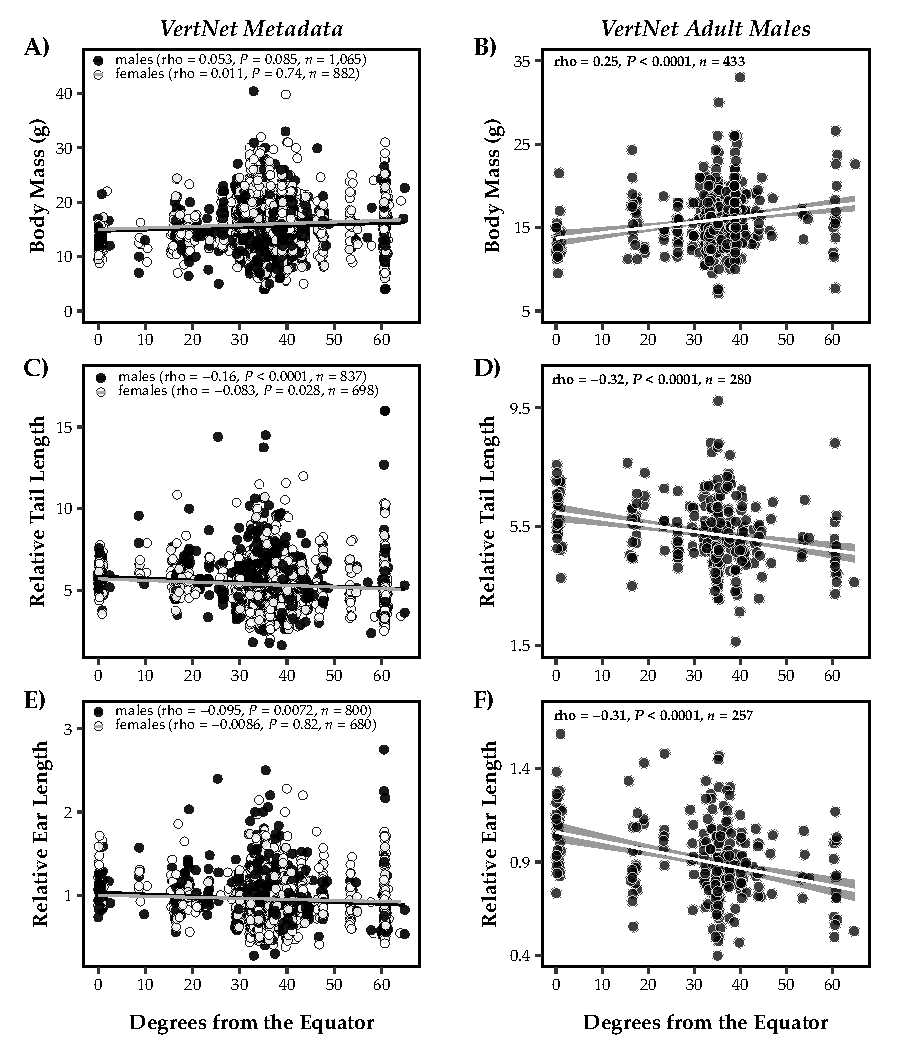
\includegraphics{../results/figures/VertNet_relative.pdf}

\textbf{Figure 1. Bergmann's rule and Allen's rule in house mice from
North and South America.} Associations between body mass (A-B), tail
length (C-D), ear length (E-F), and absolute latitude across wild-caught
North and South American house mice. Tail length and ear length are
plotted relative to body mass for each individual. Individuals are
represented as individual points, with males denoted in black and
females denoted in white. Results from Spearman correlations are
presented in each plot, along with sample sizes. For clarity, standard
error shading is ommitted from linear regression lines associated with
the VertNet Metadata (panels A, C, and E).

\newpage

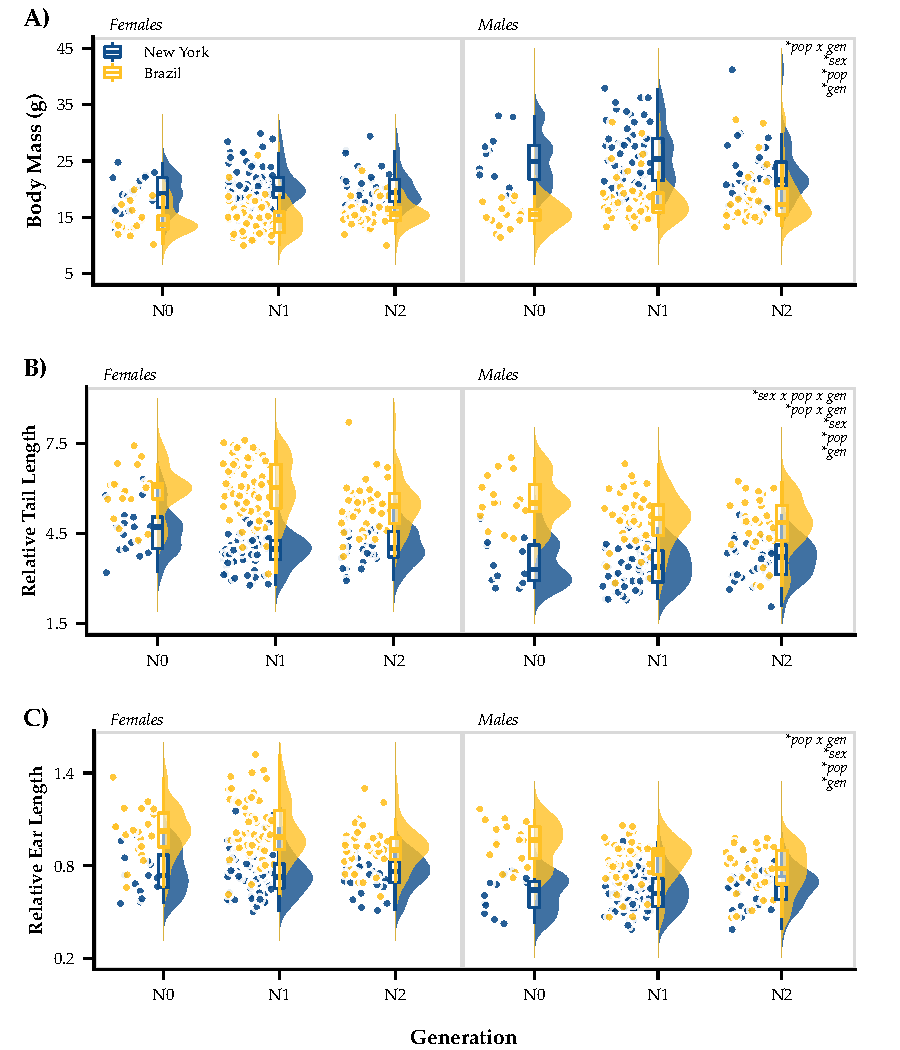
\includegraphics{../results/figures/Generations_relative.pdf}

\textbf{Figure 2. Body mass and tail length differences among
populations persist over generations in a common lab environment.}
Differences in body mass (A), tail length (B), and ear length (C)
between New York mice (blue) and Brazil mice (gold) across generations.
Tail length and ear length are plotted relative to body mass for each
individual. Population-level data are depicted as boxplots overlayed on
density plots, with boxplot vertical lines denoting 1.5x the
inerquartile range. Individuals are represented as individual points,
and the horizontal variation within each generation determined
randomally to separate points. Results from linear models are presented
in each plot (*P\textless{}0.05; Figure S1). Sample sizes: (A) n = 441;
(B) n = 432; (C) n = 434.

\newpage

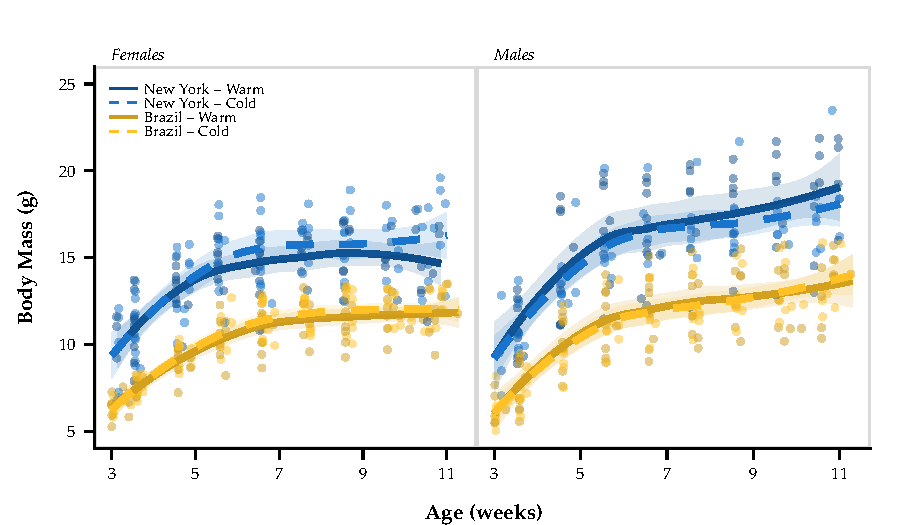
\includegraphics{../results/figures/Weekly_BW.pdf}

\textbf{Figure 3. Evolved differences in body mass across 11 weeks of
development.} Body mass growth trajectories across environments in New
York (blue) and Brazil (gold) house mice. Cold-reared mice are denoted
as dotted lines and warm-reared mice are denoted as solid lines.
Individuals are plotted as semi-transparent points (n = 80), with
population means depicted as smoothed regression fits, with standard
error shading. The same individuals depicted here are also depicted in
Figure 4.

\newpage

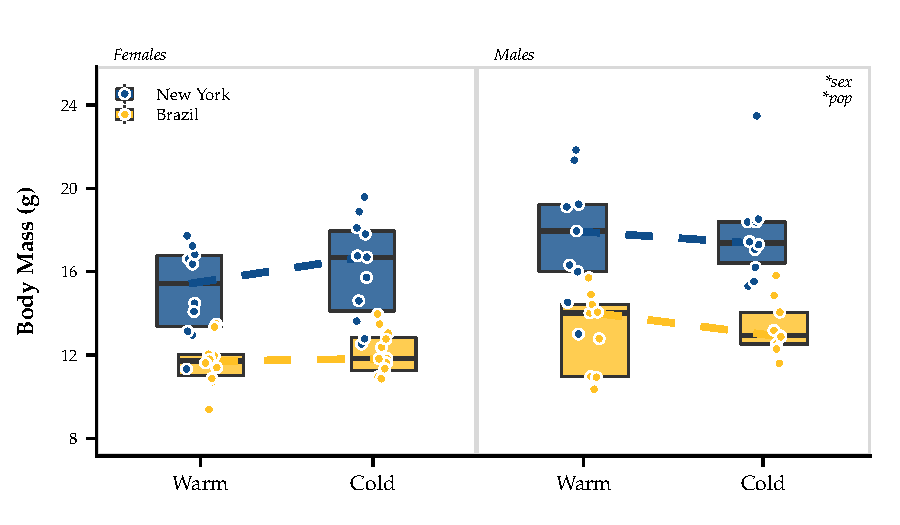
\includegraphics{../results/figures/RXNs_BW.pdf}

\textbf{Figure 4. Evolved differences and very little plasticity in body
size among New York and Brazil house mice.} Individuals are represented
as individual points (n = 80), with New York mice denoted in blue and
Brazil mice denoted in gold. Boxplots indicate the 25th, median, and
75th quartiles. Results from linear mixed models are presented in each
plot (*P\textless{}0.05; Figure S2). The same individuals depicted here
are also depicted in Figure 3.

\newpage

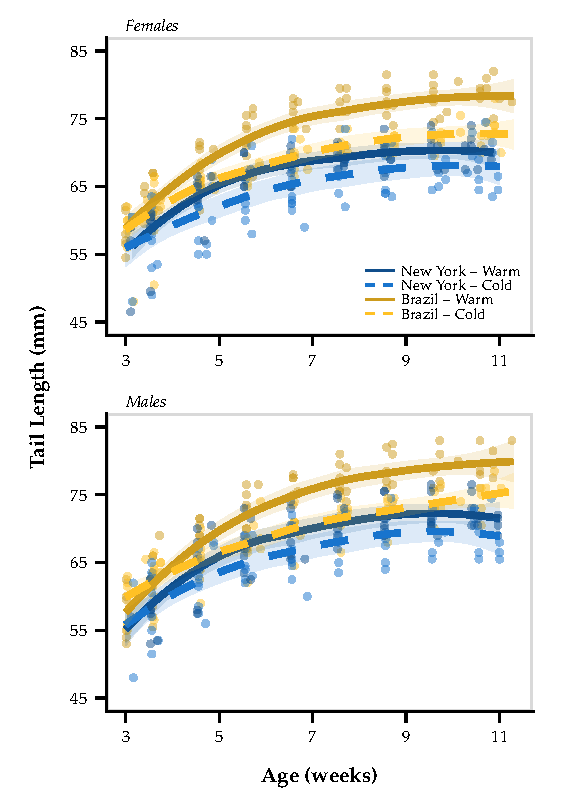
\includegraphics{../results/figures/Weekly_Tails.pdf}

\textbf{Figure 5. Tail length is highly influenced by cold temperature
across development.} Absolute tail length growth trajectories across
environments in New York (blue) and Brazil (gold) house mice.
Cold-reared mice are denoted as dotted lines and warm-reared mice are
deonted as solid lines. Individuals are plotted as semi-transparent
points (n = 80), with population means depicted as smoothed regression
fits, with standard error shading. The same individuals depicted here
are also depicted in Figure 6.

\newpage

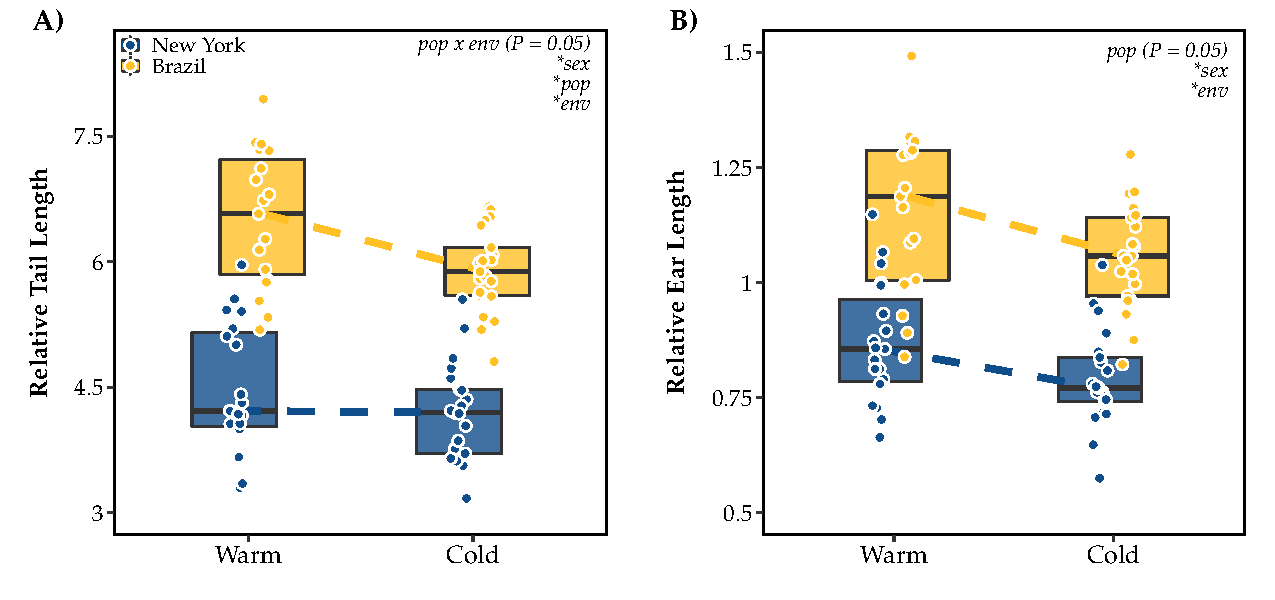
\includegraphics{../results/figures/RXNs_Extremities_relative.pdf}

\textbf{Figure 6. Adaptive phenotypic plasticity in extremity length
among New York and Brazil house mice.} Relative tail length (A) and
relative ear length (B) were calculated by regressing from body mass.
Individuals are represented as individual points (tail length: n = 80;
ear length: n = 78), with New York mice denoted in blue and Brazil mice
denoted in gold. Boxplots indicate the 25th, median, and 75th quartiles.
Both sexes were combined for simplicity. Results from linear mixed
models are presented in each plot (*P\textless{}0.05; Figure S2). The
same individuals depicted here are also depicted in Figure 5.

\newpage

\hypertarget{supplemental-figures}{%
\subsection{Supplemental Figures}\label{supplemental-figures}}

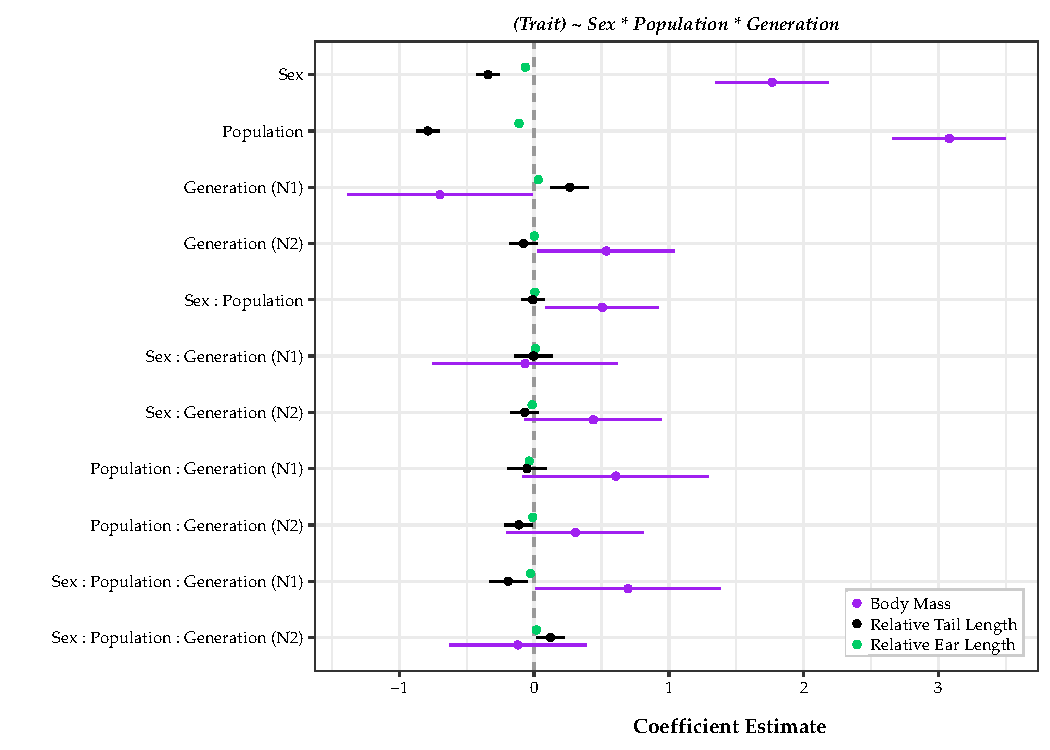
\includegraphics{../results/figures/GenerationsModel_relative.pdf}

\textbf{Figure S1. Effect sizes for common garden experiment one,
investigating the fixed effects of sex, population, and generation on
body mass, tail length, and ear length.} Points and ranges represent
model estimates and 95\% credibility estimates for the linear model,
with color indicating the phenotypic trait (purple: body mass; black:
tail length; green: ear length). Solid lines that do not cross the
dotted, vertical line are significant.

\newpage

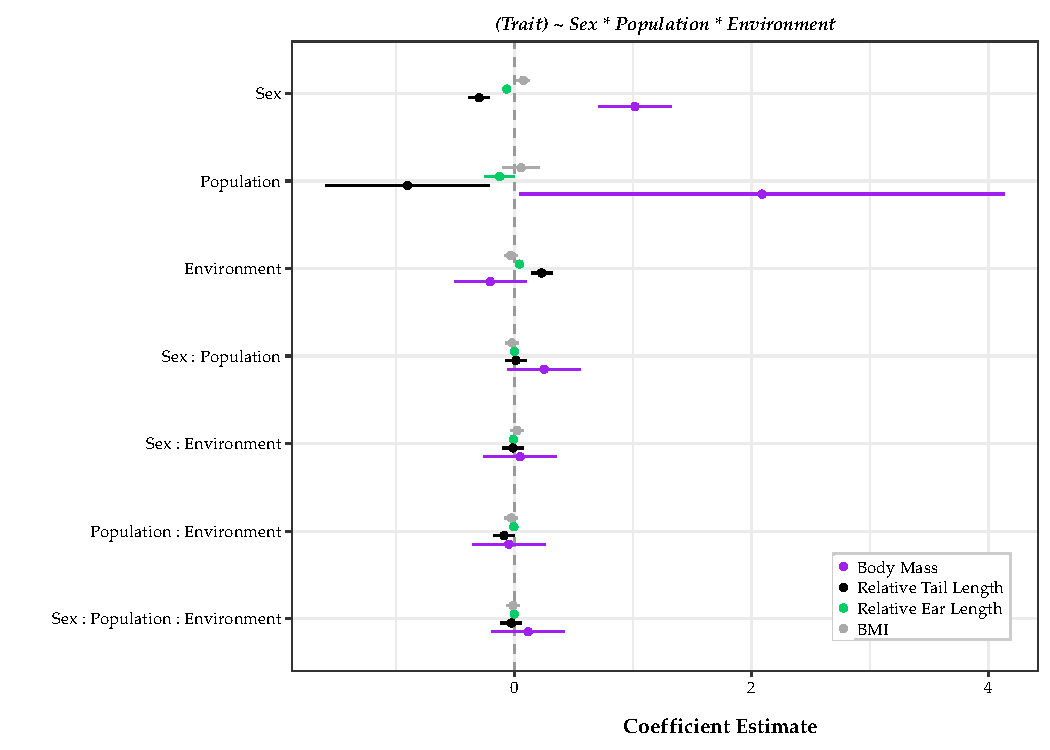
\includegraphics{../results/figures/RXNsModel_relative.pdf}

\textbf{Figure S2. Effect sizes for common garden experiment two,
investigating the fixed effects of sex, population, and environment on
body mass, tail length, and ear length.} Points and ranges represent
model estimates and 95\% credibility estimates for the linear mixed
model, with color indicating the phenotypic trait (purple: body mass;
black: tail length; green: ear length; gray: BMI). Solid lines that do
not cross the dotted, vertical line are significant.

\newpage

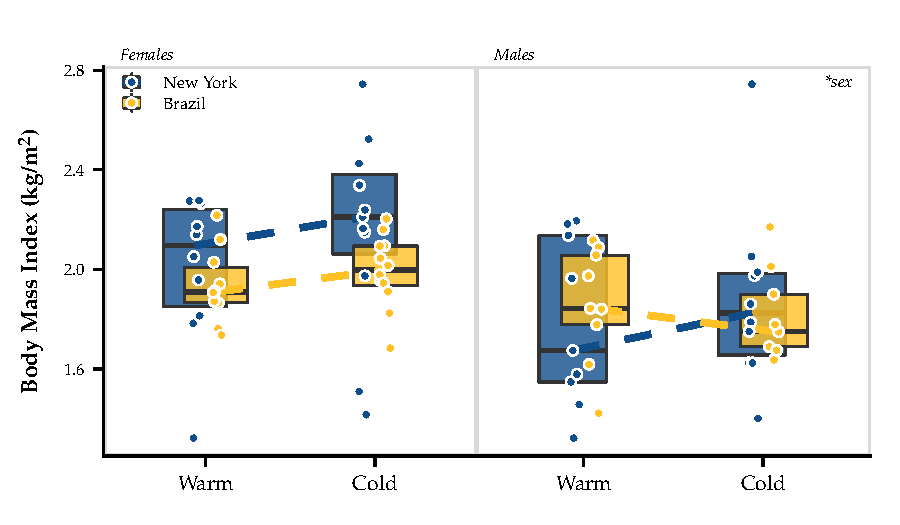
\includegraphics{../results/figures/RXNs_BMI.pdf}

\textbf{Figure S3. No differences in body mass index (BMI) among New
York mice and Brazil mice.} No evolved differences or plasticity in BMI
between New York (blue) and Brazil (gold) house mice. Individuals are
represented as individual points (n = 80).

\end{document}
